% chapter2.tex

\chapter{Simple Clouds Model}  
\label{ch:chapter2}


In this chapter, the literature about clouds and cloud schemes will be reviewed. The roles of clouds in climate system is reviewed in Section \ref{sec:chp2_role_of_clouds}. A brief history of cloud scheme development is reviewed in  \ref{sec:chp2_cld_scheme}

%\epigraph{\textit{Let's begin the scientific journey!}}{\textit{Qun Liu}, 2018}

\section{Roles of clouds in climate system}
\label{sec:chp2_role_of_clouds}
% Literature review about the role of clouds in climate system

Clouds usually cover more than half areas of the Earth at any given time \citep{Houze2014} and play a fundamental role in Earth's radiation budget and hydrological cycle. In general, clouds can reflect the sunlight (shortwave radiation) back into space and absorb the longwave radiation emitted from the surface, part of which will return to the surface. In general, the net effect of cloud is to cool the earth comparing to the cloud-free conditions. According to \cite{Zelinka2017}, the net cooling effect of clouds is about 18 Wm$^{-2}$, which is roughly five times as large as the heating effect of doubling CO$_2$. Therefore, even a small change of clouds could have large influence to the climate, that's one possible reason that why the cloud feedback is so important in climate system. 


\subsection{Cloud feedback}

\begin{figure}[h]
	\centering
	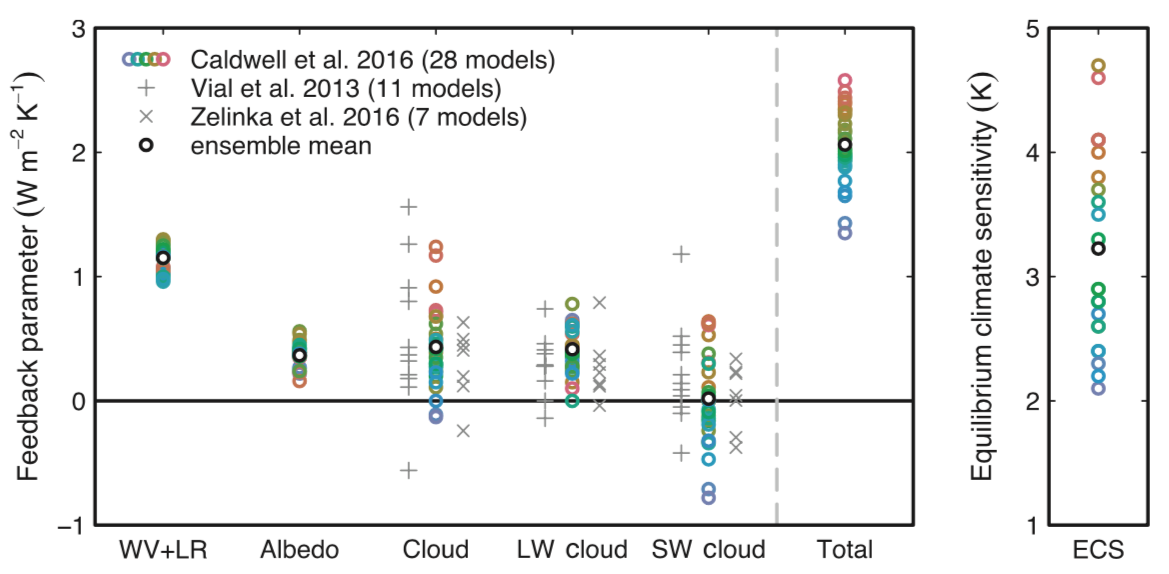
\includegraphics[width=1\linewidth]{{figs/chp2/cloud_feedback_ceppi}.png}
	\caption{Strengths of individual global-mean feedbacks and equilibrium climate sensitivity (ECS) for CMIP5 models, derived from coupled experiments with abrupt quadrupling of CO$_2$ concentration. Circles are colored according to the total feedback parameter. The Planck feedback (mean value of -3.15 W m$^{-2}$ K$^{-1}$) is excluded from the total feedback parameter shown here. Adapted from \cite{Ceppi2017}.}
	\label{fig:cld_feed_back_ecs}
\end{figure}

Cloud feedback is the variation of cloud radiative forcing at top-of-atmosphere (TOA) in response to global warming. In the fifth assessment report of the Intergovernmental Panel on Climate Change (IPCC AR5), the sign of net cloud radiative feedback is likely positive with an estimate of 0.6 Wm$^{-2}$K$^{-1}$ \citep{stocker2013climate}, which, however, has a lot of uncertainties (-0.2 to 2 Wm$^{-2}$K$^{-1}$). As shown in Figure \ref{fig:cld_feed_back_ecs}, comparing to the water vapor, lapse rate and albedo feedbacks, cloud feedback have the largest spread, which in fact is the largest uncertainty of simulated climate response to CO$_2$ foricng (i.e. climate sensitivity) in the general circulation models (GCMs) \citep{Ceppi2017}. Lots of efforts have been payed to investigate the possible reasons for the uncertainty of cloud feedbacks. For example, \cite{Webb2015} has proposed the Selected Process On/Off Klima Intercomparison Experiment (SPOOKIE) project, where the role of the convection has been accessed in the first phase of the project. They conclude that while parametrized convection influences the strength of the cloud feedbacks substantially in some models, other processes must also contribute substantially to the overall inter-model spread. In the second phase, the roles of cloud scheme will be examined. %, where the cloud fraction, cloud water content and effective cloud droplets radius are prescribed or will be diagnosed empirically.

A recent study by \cite{Sherwood2020} estimates that total cloud feedback is 0.45 Wm$^{-2}$K$^{-1}$ and the uncertainty (0.12 to 0.78 Wm$^{-2}$K$^{-1}$) is narrowed compared to the results from IPCC AR5. Nevertheless, the uncertainty of cloud feedback is still the largest ones among all the feedback parameters (see Table 1 of \citealt{Sherwood2020}), which has no clear reduction from CMIP5 to CMIP6 (see Figure 4 of \citealt{Sherwood2020}).

\subsection{Coupling with circulation}


%\section{Cloud Radiative Effect and its feedback}

%\section{Method: Diagnosis of cloud}

\section{Cloud schemes}
\label{sec:chp2_cld_scheme}

\begin{figure}[h]
	\centering
	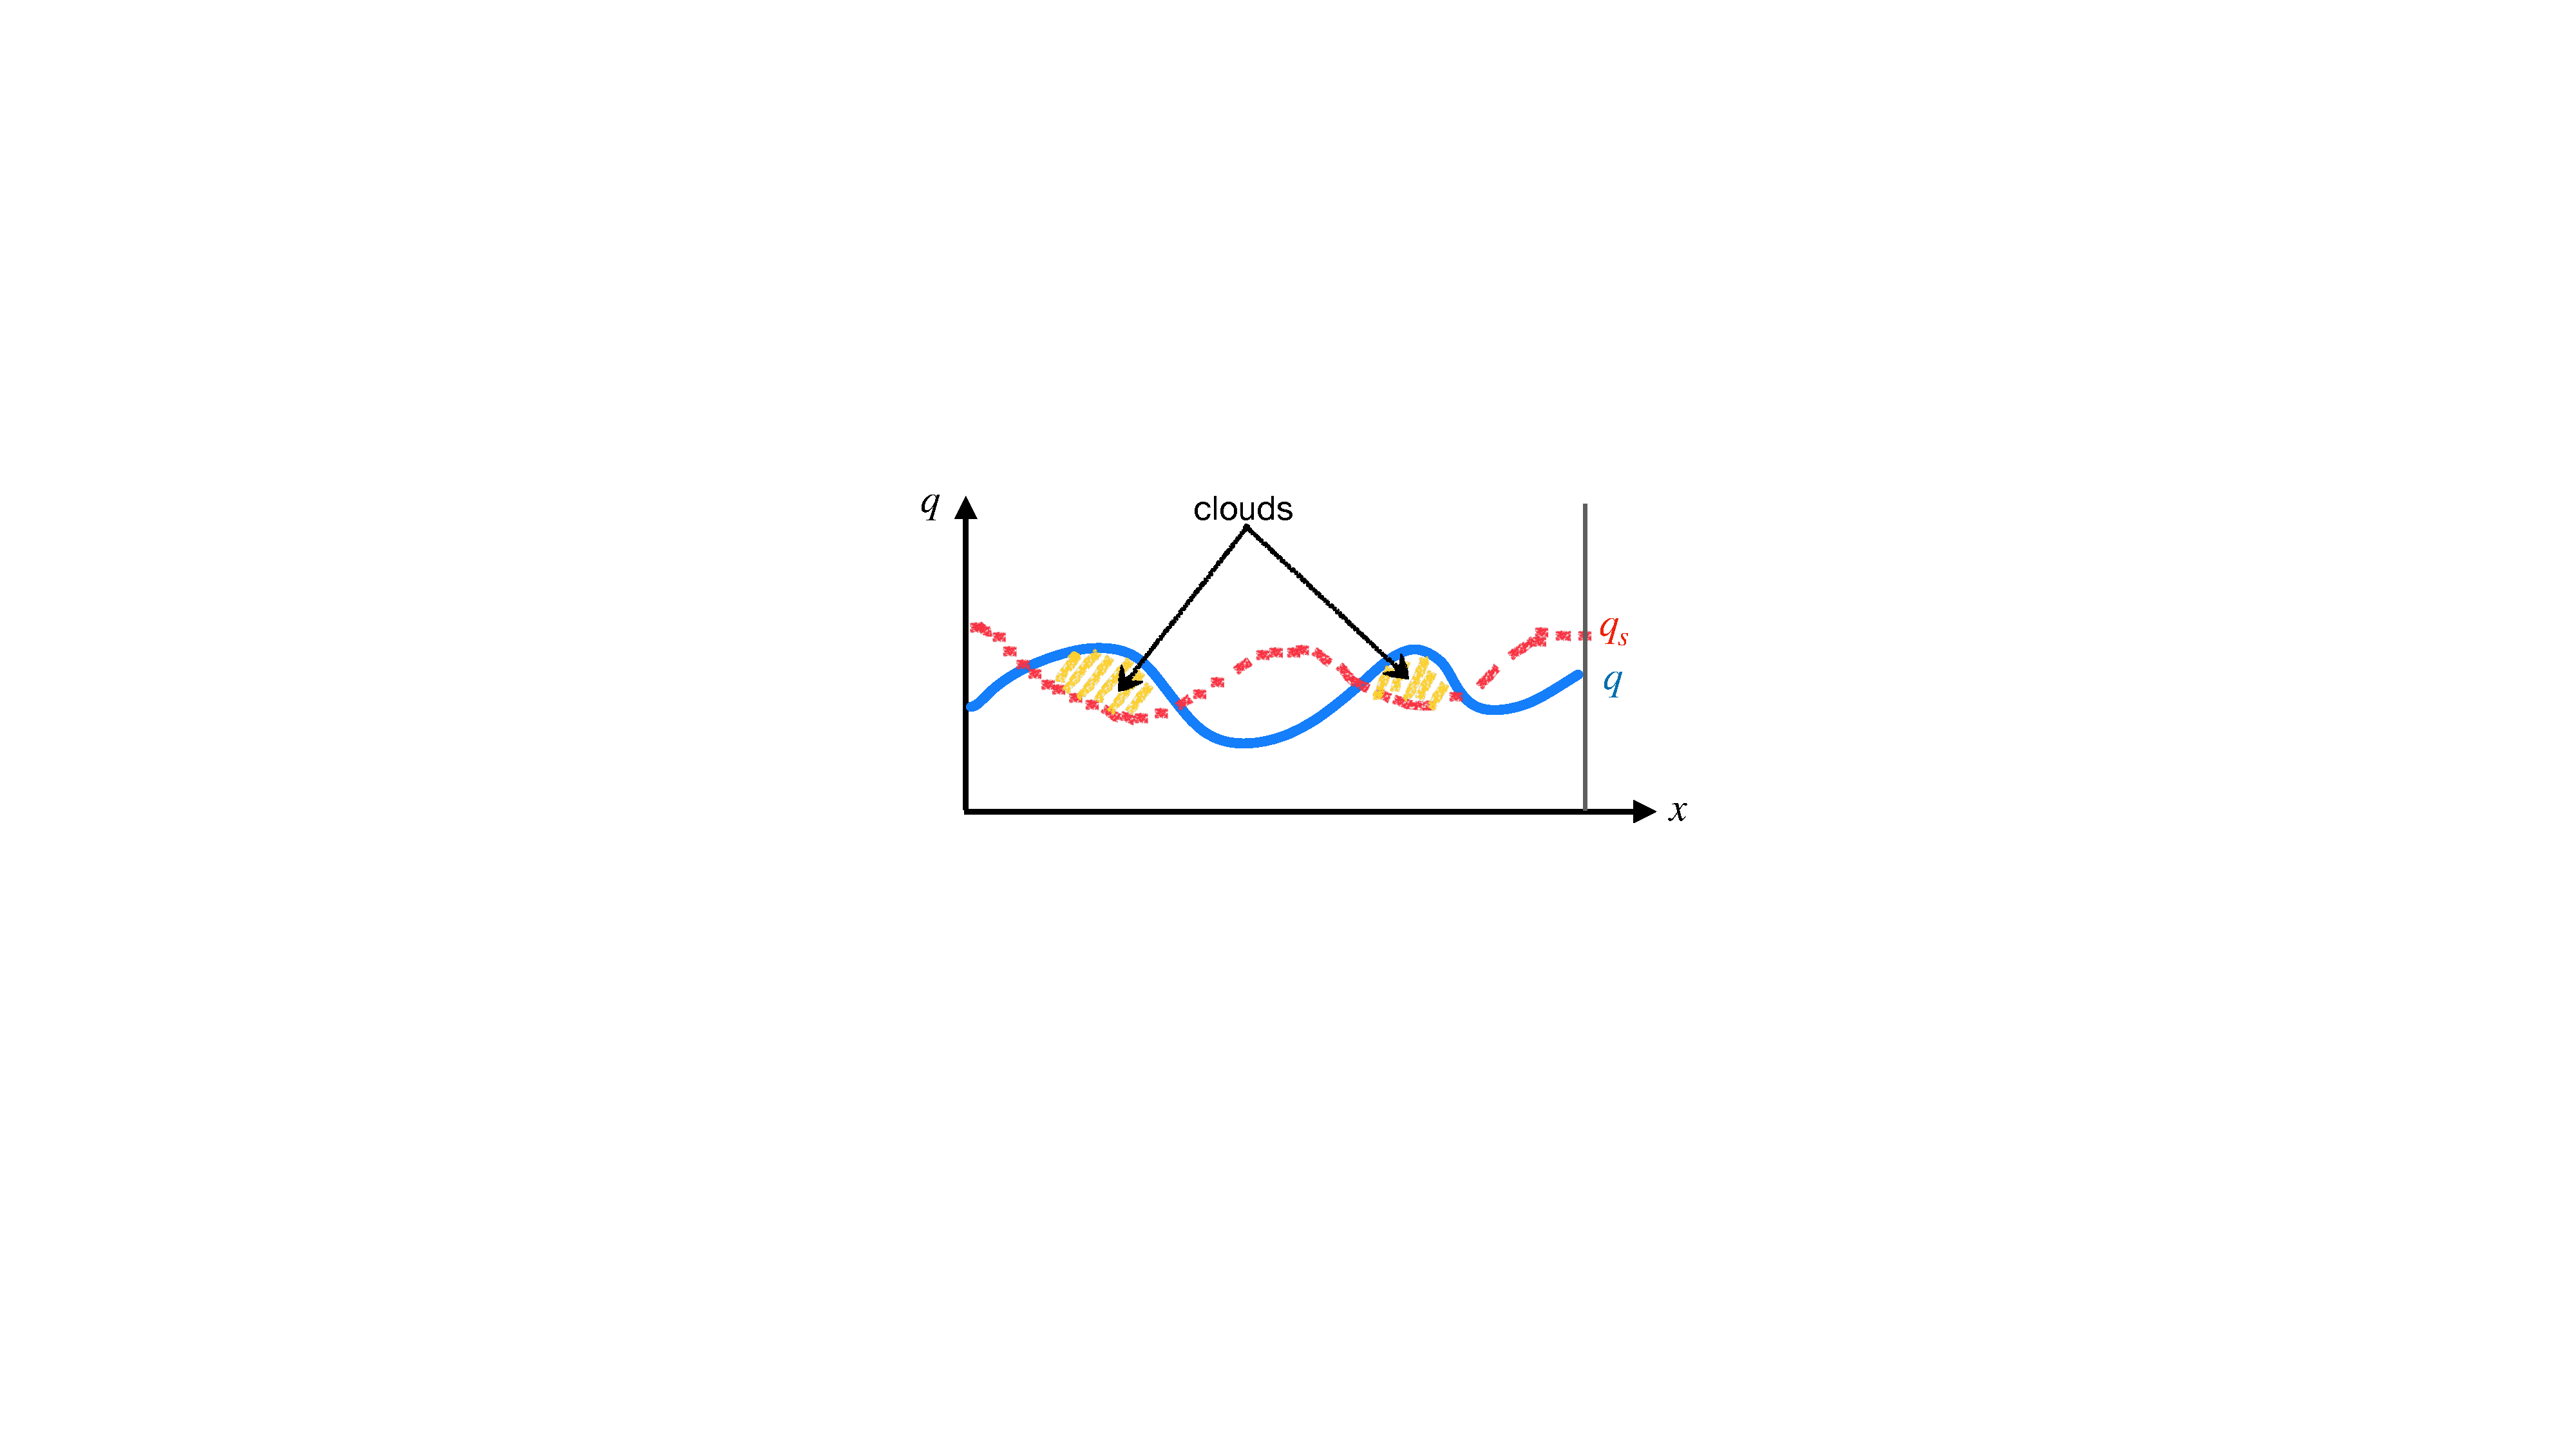
\includegraphics[width=0.8\linewidth]{{figs/chp2/Schematic_partial_cloud_cover_in_gridbox}.pdf}
	\caption{Schematic showing that partial cloud cover in a grid box (1D) when temperature or humidity fluctuations exist. The blue line shows humidity and the red dashed line indicates saturation mixing ratio of the grid box. The shaded regions are cloudy parts as the humidity exceeds the saturation mixing ratio.}
	\label{fig:schematic_partial_clouds}
\end{figure}

At present the typical horizontal resolution of the GCMs is 50-200km, but the clouds usually involve the air motions in mesoscale and convective scale \citep{Houze2014}, which are usually in sub-grid scale both horizontally and vertically, implying that cloud processes are hard to be explicitly resolved by the GCMs. In this case, the ``parameterization" becomes a practical way to build cloud schemes. The parameterization is to represent the effects of the smaller-scale processes (turbulence, cloud microphysics, convection, etc.) in terms of the large-scale states (such as velocity, temperature, pressure, humidity) \citep{Randall2003}, which could be seen as a way to find potential relationships between the unknown and known variables \citep{Randall1989}.

Previous studies have investigated various ways to represent clouds in climate models. For example, \cite{Holloway1971} prescribed the clouds externally with climatological data without dynamic interplay with the other components of the model. Some early modelling studies made the assumption that a grid box in the model is either fully saturated or totally unsaturated. However, this assumption is not reasonable enough as the humidity can distribute unevenly within a grid box, suggesting that condensation can occur even the relative humidity is less than 100\%. A general idea is to link the cloud cover with the relative humidity, as one can expect that the amount of condensation would increase with the increase of mean humidity of the model grid box, which is the basis for some diagnostic methods.

Diagnostic schemes predict the cloudiness based on the model variables empirically or statistically. In these schemes, the clouds can be linked to atmospheric outputs such as relative humidity, vertical velocity and static stability, among which the linear relationship between cloud fraction against RH could be simplest one. For example, \cite{Smagorinsky1960} found empirically that non-convective cloud amount correlated with the average relative humidity in the respective layers (Figure \ref{fig:Smagorinsky_RH_cld}), arguing that the non-precipitating condensation depend only on the accumulated history of vertical motion, which can be reflected by the humidity. \cite{Ricketts1973} obtained roughly linear relationship between cloud amount and observed relative humidity but commented that the relationship is somewhat indefinite.

Water vapor generally distributes heterogeneously in the grid box, so the averaged RH within a box should be less than 1 for a partial coverage of clouds. Previous studies usually adopt the critical relative humidity $RH_{crit}$ as the minimum threshold for clouds to form, which is often left as a free parameter that can be tuned during model development (e.g. \citealp{Hourdin2017,Kay2012,Mauritsen2012}). For example, \cite{Sundqvist1978} and \cite{Sundqvist1989} find that cloud fraction can be rewritten as a function of critical RH by assuming the water vapour is uniform distributed within the grid box. In general, $RH_{crit}$ decreases with height, but will vary according to different types of clouds. Although the $RH_{crit}$ doesn't have clear physical meaning, it can be used to modify the cloud amounts in different locations. For example, one can increase $RH_{crit}$ asymptotically to nearly unity to prevent the unrealistic circus clouds \citep{Sundqvist1989}. 

As a unique predictor, RH is very simple and useful to diagnose the cloudiness, and it is still widely used in GCMs \citep[e.g.,][]{Gordon1992,Park2014,Pope2000}. However, it is not valid for all the cases. As we can see, some studies also made use of other variables to diagnose the cloudiness. For instances, \cite{Xu1996} developed a semi-empirical scheme to determine the stratiform cloud fraction based on grid-averaged mixing ratio of condensate (cloud water and cloud ice) and RH. As for the scheme provided by \cite{Slingo1987}, both the RH and vertical velocity were taken into account, in which different empirical relations were used for different clouds including low, middle, high and convective clouds.

In summary, the methods based on relative humidity and other predictors are useful to diagnose the cloudiness, which ensures that the clouds can form before the grid box get saturated. One problem for the diagnostic methods is that in most cases the cloud condensate has to be diagnosed or prognosed via other methods \citep[e.g.,][]{Zhang2003, Park2014}, which could lead to some inconsistencies between cloud fraction and cloud condensate (e.g. \citealp{Gregory2002, Tompkins2005}).

\begin{figure}
	\vspace{-0.3cm}
	\centering
	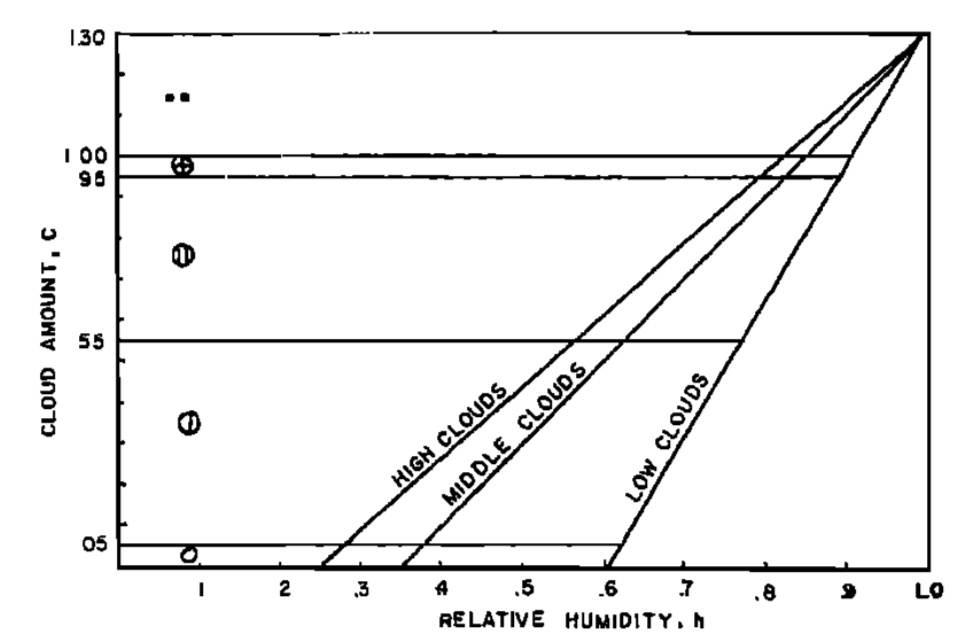
\includegraphics[width=0.6\linewidth]{{figs/chp2/Smagorinsky1960}.png}
	\caption{Empirically determined relation of mean relative humidity $h$ in the layers 1000-800mb, 800-550mb and 550-300mb with cloud amount $c$ classed as low, middle and high clouds. Adapted from Figure 1 of \cite{Smagorinsky1960}.}
	\label{fig:Smagorinsky_RH_cld}
\end{figure}

In contrast, the prognostic approach \citep[e.g.,][]{Tiedtke1993} is to explicitly calculate the clouds related variables, such as cloud water content, in order to pursuing a unification of all clouds processes, which is more realistic in some degree and requires more physical basis and interactions with other parts of the models. Another widely used cloud prediction method is statistical scheme, in which the cloud fraction and in-cloud liquid water/ice are determined based on the assumed probability distributions of subgrid variability of thermodynamic properties. As the cloud related variables such as moisture and temperature are not the same everywhere but distributed randomly within the grid box, it is natural to assume that the cloud cover depends on the distribution of moisture, sometimes on the joint distribution of moisture and temperature. As shown in a very early work, \cite{Sommeria1977} gave up the assumption that a grid is either entirely saturated or unsaturated in the climate models and proposed the idea to use the statistical distribution of moisture within the grid box. For example, given the probability distribution function (PDF) of the total water ($q_t$ is the mixing ratio) in grid box, the cloud fraction ($CF$) can be caluculate as $CF=\int_{q_s}^{\infty}PDF(q_t)\operatorname{d}q_t,$
and the cloud water content ($q_c$ is the mixing ratio of cloud water) is
$q_c=\int_{q_s}^{\infty}(q_t-q_s)PDF(q_t)\operatorname{d}q_t,$ where $q_s$ is the saturation mixing ratio in both formulations.

However, the shapes of subgrid-scale PDF of total water specific
humidity, saturation deficit, or a combined variable of liquid water and potential temperature are difficult to determine due to limit of observational data, so sometimes the model data are also used \citep{Bony2001}. Additionally, many different forms PDF have been proposed in the previous studies. For example, \cite{LeTreut1991} made use of the uniform distribution of total water in the grid box to calculate the clouds cover and liquid water content. Other symmetrical distributions, such as Gaussian distribution \citep{Sommeria1977}, triangular distribution \citep{Smith1990} and skewed distributions, such as lognormal distribution \citep{Bony2001} and beta distribution \citep{Tompkins2002}, have also been employed in numerical models. However, there are also some problems in the distributions. For example, the Gaussian distribution is unbounded, indicating that the maximum cloud condensate mixing ratio might approach infinity, and cloud cover is always large than zero \citep{Tompkins2002}. In general, complicated forms of the PDF need more parameters to fit. But due to the limitation of the data, it is possibly hard to validate the distributions. Linking the statistical cloud scheme to other physical processes seems a promising way to improve cloud simulations. For example, \cite{Qin2018} developed a Gaussian PDF cloud scheme with the PDF variance diagnosed from the turbulent
and shallow convective processes, which could improve the simulation of low marine clouds and alleviate double Intertropical Convergence Zone (ITCZ) problem \citep{Qin2018alleviated}.

The statistical cloud schemes may have better performance than the diagnostic ones, but considering the fact that there is no clouds scheme in Isca currently, it would be useful to implement the simple diagnostic schemes in Isca first, which can be seen as the first step to implemented a hierarchy of cloud schemes.
